\section{Implementação de Hardware}

\subsection{Sensor de Temperatura}

O sensor de temperatura DS18b20 é alimentado pelos pinos de 5V e GND (terra) do microcontrolador. seu sinal de leitura é enviado para uma porta digital, sendo utilizado um resistor de 4,7 k$\omega$ como pull up, caso exista uma leitura errada do sensor. A figura \ref{figura:micro_temp} ilustra a conexão do microcontrolador com o sensor de temperatura. 


\begin{figure}[h]
    \centering
    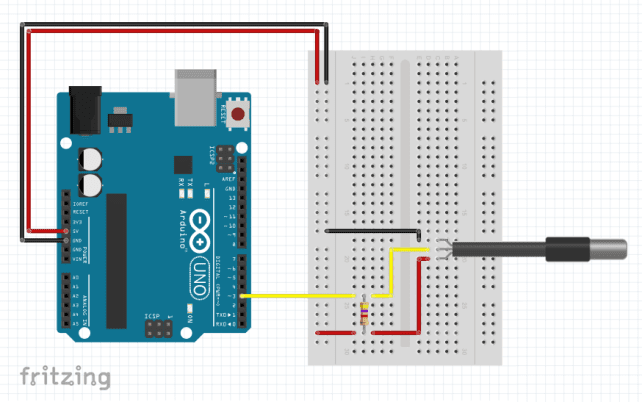
\includegraphics[scale=0.40]{figuras/implementacao/hardware/DSsensor.png}
    \caption{Esquema de conexão entre microcontrolador e sensor de temperatura DS18B20.}
    \label{fig:micro_temp}
\end{figure}


O excerto de código em linguagem Arduino a seguir representa a função utilizada para ler o valor de saída do sensor. A biblioteca OneWire implementa o protocolo proprietário de comunicação serial da Dallas Semicondutor, fabricante do sensor. Ela é utilizada em conjunto com a biblioteca livre DallasTemperature para estabelecer a comunicação com o DS18B20.

% // TODO: Referências das bibliotecas
% https://github.com/milesburton/Arduino-Temperature-Control-Library
% https://github.com/PaulStoffregen/OneWire

% \begin{lstlisting}[language=C]

% #include <OneWire.h>
% #include <DallasTemperature.h>
% #define ONE_WIRE_BUS D6

% OneWire oneWire(ONE_WIRE_BUS);
% DallasTemperature sensors(&oneWire)

% void setup() {
%     sensors.begin();
% }

% float readTemperature() {
%     return sensors.getTempCByIndex(0);
% }

% \end{lstlisting}


\subsection{Sensor de pH}

O sensor de pH é conectado a um circuito auxiliar que trata o sinal proveniente da ponta de prova. Esse circuito é conectado aos pinos de 5V e GND do microcontrolador para alimentação, e envia do dado coletado por meio de sinal analógico, como observado na figura \ref{fig:micro_ph}. 


\begin{figure}[h]
    \centering
    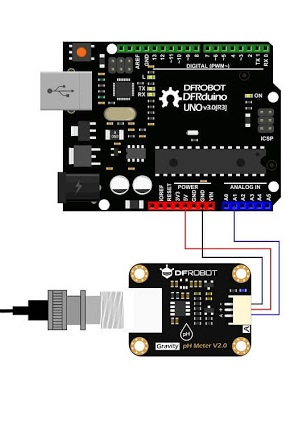
\includegraphics[scale=0.65]{figuras/implementacao/hardware/micro_ph.jpg}
    \caption{Esquema de conexão entre microcontrolador e sensor de pH E-201-C.}
    \label{fig:micro_ph}
\end{figure}


Para utilização desse sensor, é necessário sua calibração, que consiste na medição da tensão de saída do sensor em soluções com diferentes concentrações de \(H^+\) e obtenção de uma equação linear que traduza a voltagem medida em um valor de pH. Para isso utilizadas soluções tampão com pH iguais a 4, 7 e 10. A calibração seguiu o seguinte processo:
\begin{enumerate}
    \item Com a solução de pH igual a 7, ajustar o ganho do circuito (por um potenciômetro) até que a leitura de voltagem seja 2,5 Volts. Essa tensão foi escolhida de forma a coincidir valor médio da tensão de alimentação do circuito com o valor médio da escala de pH;
    \item Capturar a tensão medida nas soluções com pH 4 e 10;
    \item Aplicar regressão linear, minimizando a soma dos erros quadráticos, obtendo a reta que relaciona a tensão medida com o pH da solução
\end{enumerate}


Com os valores obtidos na tabela \ref{tab:calibra_ph}, foi obtida a equação linear \ref{eq:pH}.

\begin{equation}
    pH = 2.0171 * Voltagem + 1.7152
    \label{eq:pH}
\end{equation}


\begin{table}[H]
    \begin{center}
        \begin{tabular}{ |c|c| } 
            \hline
            Voltagem & pH \\
            \hline
            2.50 & 7.0 \\ 
            \hline
            1.20 & 4.0 \\ 
            \hline
            4.16 & 10.0 \\ 
            \hline
        \end{tabular}
        \caption{\label{tab:calibra_ph}Medições de tensão em soluções tampão para calibração do sensor de pH.}
    \end{center}
\end{table}


A leitura do pH medido pelo sensor pelo microcontrolador segue o seguinte algoritmo:
\begin{enumerate}
    \item Valor inteiro entre 0 e 1024 recebido pelo sensor é lido na porta analógica;
    \item Valor lido é convertido em uma diferença de tensão seguindo \(Voltagem = medida * 5 / 1024\);
    \item Diferença de tensão é convertida na leitura de pH seguindo equação linear obtida na calibração do sensor.
\end{enumerate}


% \begin{lstlisting}[language=C]

% int ph_pin = A0;

% float readPH() {
%     int measure = analogRead(ph_pin);
%     double voltage = measure * 5 / 1024;
%     return 2.0171 * voltage + 1.7152;
% }

% \end{lstlisting}


\subsection{Conexão e Comunicação do Microcontrolador}

Com os sensores propriamente conectados e calibrados, o microcontrolador foi configurado para se conectar à Internet através de conexão WiFi e a enviar os dados coletados por meio do protocolo MQTT. O Wemos D1 é controlada pelo módulo ESP8266, de forma que ofereça conectividade WiFi nativa. 
A biblioteca ESP8266WiFi foi utilizada para estabelecer a conexão Wifi, em conjunto com a biblioteca PubSubClient para publicar mensagens e se inscrever em tópicos MQTT. 

% https://github.com/esp8266/Arduino/tree/master/libraries/ESP8266WiFi
% https://github.com/knolleary/pubsubclient

% // TODO: Colocar código completo em Apêndice e discutir Fluxo completo aqui

\subsection{Controle de Temperatura}

Um controlador de malha fechada proporcional interativo derivativo (PID) será utilizado para controlar a temperatura do fermentador. Esse método é amplamente utilizado na indústria, possuindo boa precisão e confiabilidade, além de ser facilmente sintonizado. Inicialmente são definidos parâmetros analógicos e depois é criado o controle digital.


\subsubsection{Controlador PID}

O controlador PID utiliza 3 ações (proporcional, integrativa e derivativa) controlar a planta minimizando o erro. Sua saída pode ser definida pela equação \ref{eq:pid}. A figura \ref{fig:pid} esquematiza a malha de controle.

\begin{equation}
%     u(t) = K_pe(t) + K_i\[\int_{0}^{t} e(\tau) \, d\tau \] + K_d\dfrac{de(t)}{dt}
    u(t) = K_pe(t) + K_i  \int_{0}^{t} e(\tau) \, d\tau + K_d\dfrac{de(t)}{\, dt}
    \label{eq:pid}
\end{equation}

Na qual:

\begin{table}[H]
    \begin{center}
        \begin{tabular}{ |c|c| } 
            \hline
            Símbolo   &  Descrição  \\
            \hline
            \(K_p\)   &  ganho proporcional  \\
            \hline
            \(K_i\)   &  ganho integrativo  \\
            \hline
            \(K_d\)   &  ganho derivativo  \\
            \hline
            \(e\)   &  erro  \\
            \hline
            \(t\)   &  tempo  \\
            \hline
            \(\tau\)   &  tempo de integração \\
            \hline
        \end{tabular}
        \caption{\label{tab:variaveis_pid}Descrição das variáveis do controlador PID da Equação \ref{eq:pid}.}
    \end{center}
\end{table}

\begin{figure}[h]
    \centering
    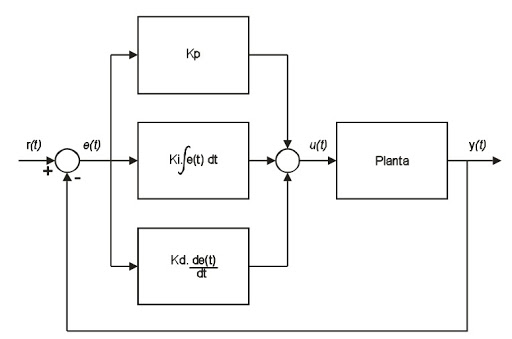
\includegraphics[scale=0.60]{figuras/implementacao/hardware/pid.jpg}
    \caption{Malha de controle PID.}
    \label{fig:pid}
\end{figure}


A ação proporcional do controlador produz um sinal de saída proporcional à amplitude do erro $e(t)$. Essa ação é útil para criar uma resposta equivalente ao tamanho do erro do sistema. A ação integral produz um sinal de saída proporcional à magnitude do erro, dependendo não só do seu valor, mas também da sua duração. Essa ação corrige o erro de off-set gerado pela ação proporcional e acelera a resposta do sistema. Por fim, a ação derivativa produz um sinal de saída proporcional à velocidade de variação do erro. Essa ação melhora a estabilidade e velocidade de resposta do sistema através de uma correção antecipada do erro. 


\subsubsection{Método de Ziegler-Nichols}


Para escolha dos parâmetros de ganho, o método de Ziegler-Nichols foi utilizado. Esse método foi escolhido principalmente pela sua simplicidade e facilidade na sintonização, visto que não é necessário uma modelagem matemática precisa da planta para o seu ajuste. 
A escolha dos parâmetros é feita a partir da observação da resposta do sistema em malha aberta com a aplicação de um degrau. A figura \ref{fig:resposta_sistema} ilustra a curva de resposta do sistema, e a tabela \ref{tab:parametros_ziegler} lista os parâmetros provenientes do método.


\begin{figure}[h]
    \centering
    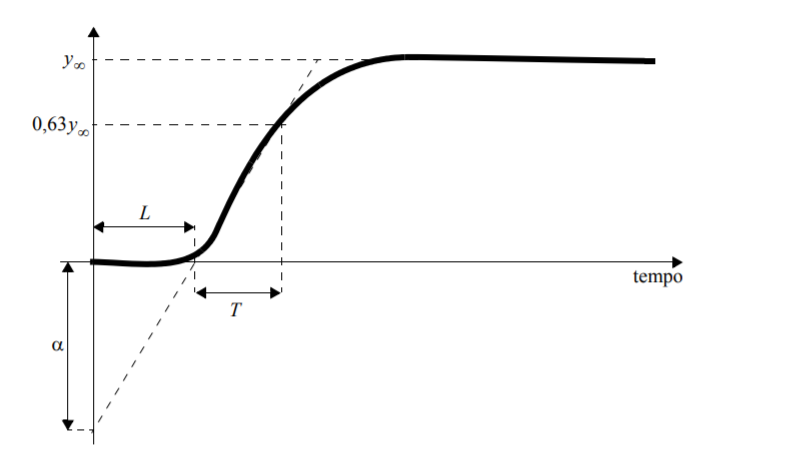
\includegraphics[scale=0.45]{figuras/implementacao/hardware/resposta.png}
    \caption{Responda do Sistema em malha aberta a sinal degrau.}
    \label{fig:resposta_sistema}
\end{figure}

\begin{table}[H]
    \begin{center}
        \begin{tabular}{ |c|c|c|c| } 
            \hline
            Controlador & \(K_p\) & \(T_I\) & \(T_D\) \\
            \hline
            \(P\) & \(1/\alpha\) &  & \\
            \hline
            \(P + I\) & \(0,9/\alpha\) & \(3L\) & \\
            \hline
            \(P + I + D\) & \(1,2/\alpha\) & \(2L\) & \(0,5L\) \\
            \hline
        \end{tabular}
        \caption{\label{tab:parametros_ziegler} Parâmetros do controlador PID seguindo método de Ziegler-Nichols.}
    \end{center}
\end{table}



\subsubsection{Anti Wind-up}


Nesta aplicação, devido a limitações do atuador, é esperado uma saturação na saída. No caso onde o sistema não consegue chegar no setpoint, teremos uma situação chamada de wind-up, na qual, a sua resposta integral irá crescer de forma indefinida. Para evitar problemas no controlador, é necessário a implementação de um sistema anti wind-up, no caso, a ação escolhida será congelar a ação do controlador em caso de saturação.  


\subsubsection*{Características do Sistema}

O objetivo do sistema é controlar a temperatura do líquido fermentado (solução de mosto e leveduras). O líquido estará dentro de um fermentador, sem entrada de ar dado que a fermentação é anaeróbica e o ar interfere na qualidade do experimento. Para expulsar o $CO^2$ gerado pela fermentação e não permitir a entrada de $O^2$ o fermentador utiliza um Air-Lock, dispositivo que funciona como válvula só permitindo a direção única desse fluxo. O fermentador será embalado em uma manta térmica, com a intenção de evitar a troca térmica com o ambiente, as seguintes trocas térmicas ocorrem no sistema. 


\begin{enumerate}
    \item A manta térmica recebe calor do ambiente através da convecção e radiação do ar. 
    \item A manta térmica transfere calor por condução para o fermentador. 
    \item O fermentador transfere calor por condução para o líquido fermentado. 
    \item O líquido fermentado produz calor pelo processo de fermentação (processo exotérmico).
\end{enumerate}


Sendo assim, o sistema com a pastilha de Peltier deve retirar do sistema uma quantidade de calor proporcional a essa recebida e gerada para manter uma temperatura estável abaixo do ambiente. Como a quantidade de calor retirada por um Peltier é proporcional a corrente, a tensão fornecida a pastilha é variada através de uma circuito ponte H que tem a sua amplitude de tensão de saída regulada por uma porta PWM.  


% \subsubsection*{Simulação do Sistema}

% Utilizando os blocos térmicos do simscape no Software Matlab, e aplicando as propriedades dos materiais é possível chegar no modelo aproximado da transmissão de calor dentro do sistema da figura \ref{fig:transcal}. Simulando o sistema no Matlab utilizando os parâmetros da tabela \ref{tab:sim_matlab}, foi obtido que éo valor a ser retirado pelo Peltierpara manter uma diferença de 10 °C entre fermentador e ambiente é de ######.


% \begin{figure}[H]
%     \centering
%     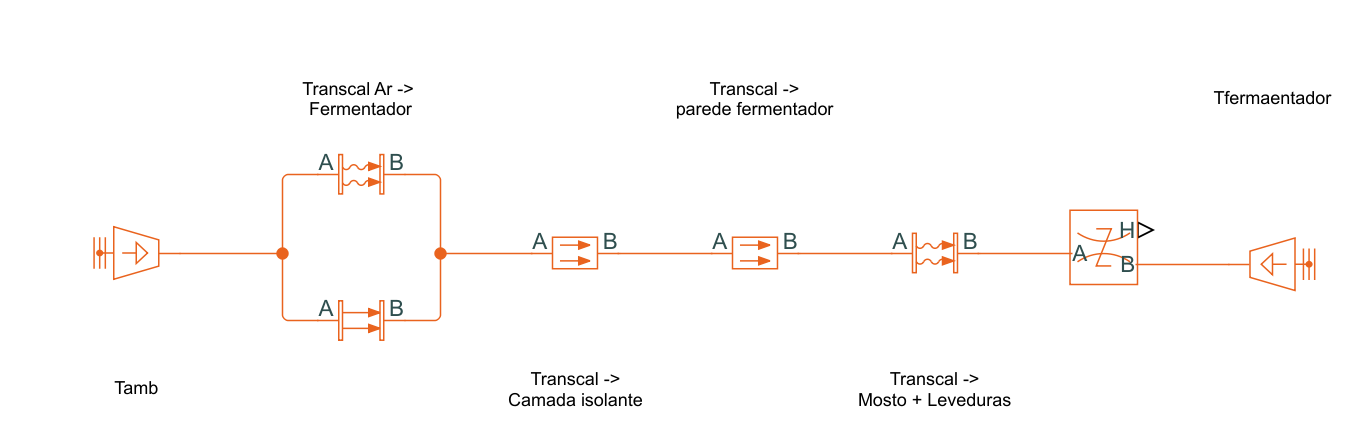
\includegraphics[scale=0.45]{figuras/implementacao/hardware/transcal.png}
%     \caption{Modelo de transmissão de calor do fermentador.}
%     \label{fig:transcal}
% \end{figure}


% \begin{table}[H]
%     \begin{center}
%         \begin{tabular}{ |c|c| } 
%             \hline
%             Parâmetro & Valor \\
%             \hline
%             Temperatura ambiente & 25 °C \\
%             \hline
%             Temperatura do fermentador & 15 °C \\
%             \hline
%             x & x \\
%             \hline
%             x & x \\
%             \hline
%             x & x \\
%             \hline
%             x & x \\
%             \hline
%             x & x \\
%             \hline
%             x & x \\
%             \hline
%             x & x \\
%             \hline
%             x & x \\
%             \hline
%             x & x \\
%             \hline
%         \end{tabular}
%         \caption{\label{tab:parametros_ziegler} Parâmetros utilizados na simulação do sistema de transferência de calor.}
%     \end{center}
% \end{table}


\subsubsection*{Circuito Ponte H}

O circuito ponte H (figura \ref{fig:ponte_h}) permite que a amplitude e sentido da tensão de entrada da pastilha de Peltier seja controlado digitalmente por um sinal PWM (Pulse Width Modulation) do microcontrolador. No Software embarcado, um valor entre 0 e 255 é utilizado para definir o duty cycle da onda quadrada do sinal PWM, como exemplificado na figura \ref{fig:pwm}. 


\begin{figure}[H]
    \centering
    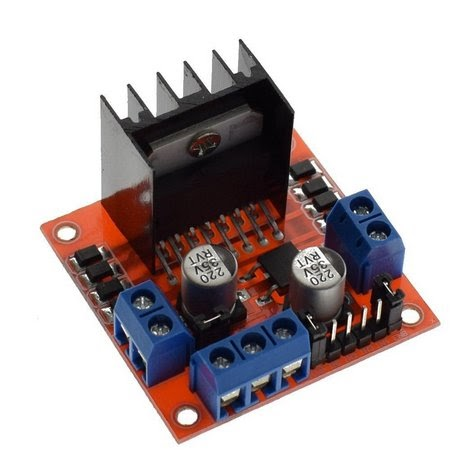
\includegraphics[scale=0.35]{figuras/implementacao/hardware/ponte_h.jpg}
    \caption{Modelo ponte H - L298N.}
    \label{fig:ponte_h}
\end{figure}

\begin{figure}[H]
    \centering
    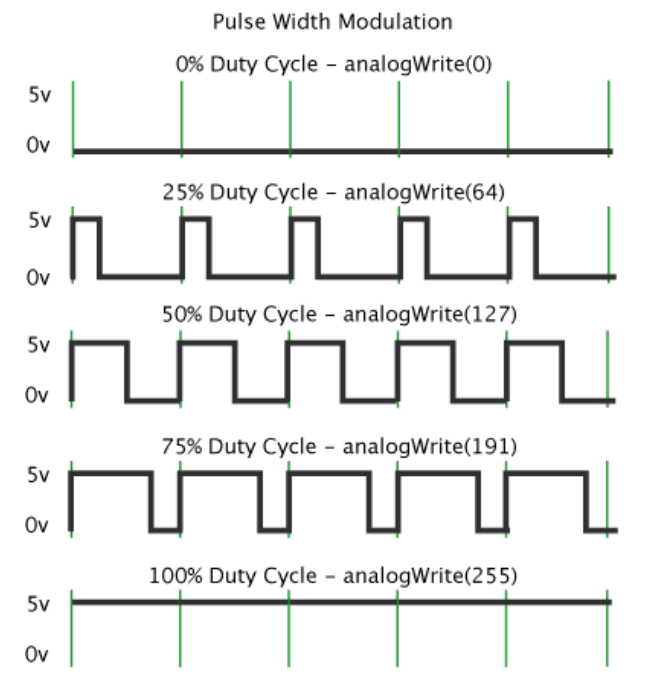
\includegraphics[scale=0.30]{figuras/implementacao/hardware/pwm.png}
    \caption{Onda quadrada do sinal PWM para alguns valores especificados no microcontrolador.}
    \label{fig:pwm}
\end{figure}


\subsubsection*{Montagem do Dispositivo}

Com as definições de controle discutidas, foi projetado o dispositivo da figura \ref{fig:dispositivo_term}, em escala aproximada. O dispositivo pode ser dividido em três partes descritas a seguir:

\begin{enumerate}
    \item Parte quente : Essa parte é ligada na face quente da pastilha e é formada por uma ventoinha e um dissipador de calor. Uma boa dissipação de calor garante uma melhor eficiência da partilha e permite que ela forneça quantidades de calor maiores para o sistema;
    \item Pastilha de Peltier: Pastilha que recebe a corrente e transforma energia elétrica em térmica. A face quente e face fria são isoladas por material isolante térmico, que ajuda na não interferência entre as partes e melhora a eficiência do sistema;
    \item Parte fria: essa parte é ligada na face fria da pastilha. Ela retira calor do sistema através de uma placa de cobra e barras de aço inox. Apesar do cobre ter uma condutividade térmica melhor, o aço inox foi escolhido para fazer a transmissão para o mosto + leveduras, por não interferir no seu gosto na exposição de pHs menores. 
\end{enumerate}


\begin{figure}[h]
    \centering
    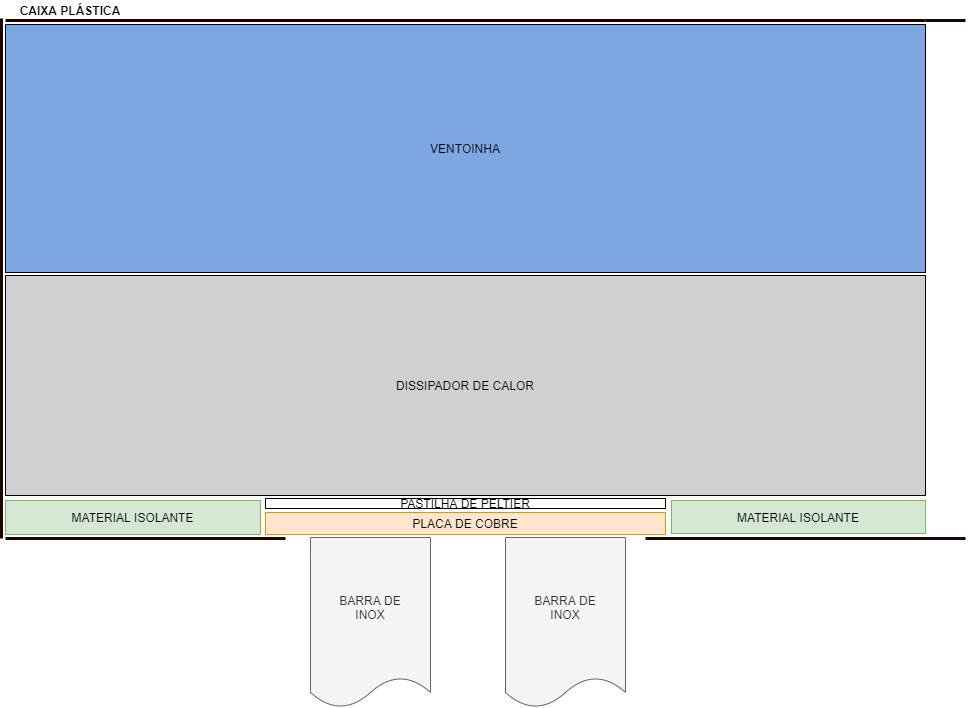
\includegraphics[scale=0.45]{figuras/implementacao/hardware/montagem.png}
    \caption{Esquema do perfil do dispositivo controlador de temperatura, escala aproximada.}
    \label{fig:pwm}
\end{figure}
